\chapter{Clustering performance evaluation}
\label{related}

The field of flat clustering algorithms is intensively addressed. Numerous metrics were created over the past years: Adjusted Rand Index(AMI) \cite{hubert1985comparing}, Adjusted Mutual Information(AMI) \cite{vinh2010information}, Homogeneity, Completeness and V-measure \cite{rosenberg-hirschberg-2007-v}, Silhouette Coefficient \cite{ROUSSEEUW198753} and many others. However, these general metrics are not directly applicable to the case of hierarchical clustering algorithms. 

This chapter will present some of the most relevant hierarchical clustering metrics. 
In the following sections of this chapter, we analyse different hierarchical clustering metrics that vary in accordance to their baseline theory, computational complexity and explainability. Some of them are strictly applicable to graphs, while others are rather for a general usage.  We compare their strength and weaknesses along with their limitations. 

\section{Graph based metrics}
Let's consider a weighted, undirected, connected graph $G = (V, E)$ of $n$ nodes, without self-loops. Let $w(i, j)$ be equal to the weight of edge $i, j$, if any, and to 0 otherwise \cite{Bonald2018a}. 
We refer to the weight of node $i$ as: $$w(i) = \sum_{j \in V}w(i,j)$$
We denote by $w$ the total weight of nodes: $$w = \sum_{i \in V}w(i)$$
Similarly, for any sets $A$, $B$ $\subset V$ , let $$w(A,B) = \sum_{i \in A, j \in B}w(i,j)$$ and $$w(A) = \sum_{i \in A}w(i)$$

\paragraph{Cluster sampling.} For every cluster pair we can calculate probability distribution as follows:
$$\forall A, B \in P, p(A,B)=\frac{{w}(A,B)}{{w}}$$ with marginal distribution 
$$\forall A \in P, p(A)=\sum_{B \in P} p(A,B)=\frac{{w}(A)}{{w}}$$

\paragraph{Dasgupta Cost.}
Recently, a new metric to evaluate the quality of hierarchical clustering was introduced by Dasgupta \cite{dasgupta2016cost} and was extended in \cite{Cohen-Addad2017}, \cite{Cohen-Addad2019}. 

Assume that a given dendrogram represents the graph $G$, a rooted binary tree $T$ whose leaves are the graph's nodes $V$. We denote by ${\cal I}$ the set of internal nodes of the tree $T$ \cite{Bonald2018a}. 
Dasgupta's cost function can be expressed as a sum over all internal tree's $T$ nodes of joint sampling probabilities of two nodes multiplied by the sum of their marginal probabilities \ref{eq:dasgupta}. 

\begin{equation}
\label{eq:dasgupta}
\sum_{A,B: (A,B) \in {\cal I}}p(A,B)(p(A) + p(B)) 
\end{equation}

The shortcomings of this method are:
\begin{itemize}
	\item It necessarily relies on the structure of a graph.
	\item It is not a continuous function of $A$ and $B$: slight changes modify the score significantly.
	\item Its main issue lies in a tie-breaking: since we have merges of equal heights in a dendrogram, it is not obvious to decide which pair of clusters to consider for merge first. Each will give a different value for Dasgupta's cost. Finding the tree that minimizes the cost function is NP-hard \cite{dasgupta2016cost}.
\end{itemize}

Since we would like to test beyond graph-based datasets, we discard this metric for the evaluation.

\section{Tree based metrics}
\paragraph{Robinson-Faulds.} \label{RF_metric}
The Robinson-Foulds (RF) distance is one of the most frequently used metrics to measure the distance between trees \cite{ROBINSON}. It measures the number of branch partitions (splits) present only in one of the trees and scores 1 for each division that is not matched. In order to move from the distance calculation to similarity, we use the formula below. 

%\begin{equation}
%\begin{split}

$$\text{RF} = 1 - \frac{\text{number of dissimilar splits}}{\text{total number of splits}}$$

%\end{split}
%\end{equation}

\begin{figure}[H]
	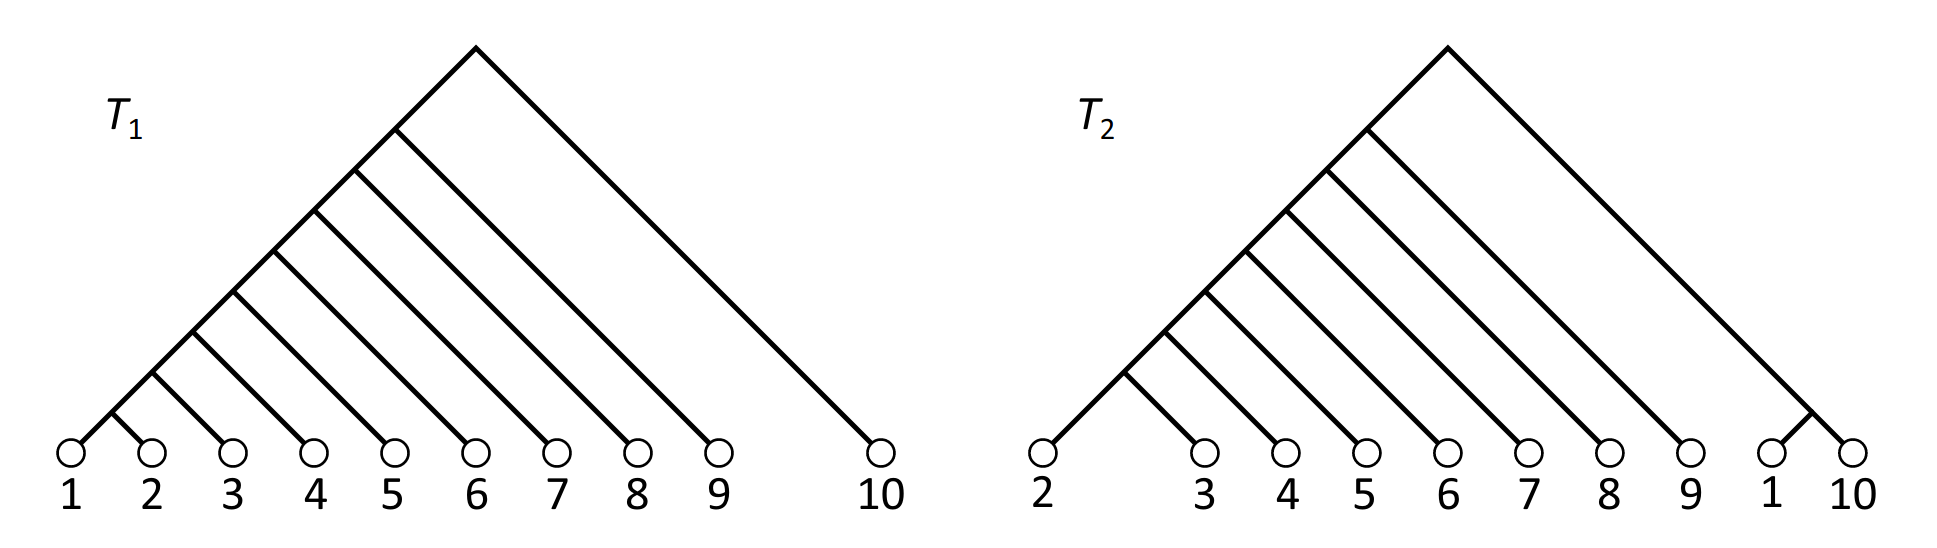
\includegraphics[width=1\textwidth,keepaspectratio=true]{figures/RF_shortcommings1.png}
	\centering
	\caption{Two rooted phylogenetic trees. Despite their high similarity, the RF metric between these two trees is equal to $\frac{1}{9}$ \cite{RF2013}.}
	\label{fig:rf_shortcommings}
\end{figure}

RF has its well-known shortcomings. For instance, moving a single node in a tree can result in a considerable jump of RF score when, in reality, these trees are almost identical as shown in Figure \ref{fig:rf_shortcommings}. 
There are numerous modifications of this metric, which are trying to address this issue \cite{Kuhner1994}, \cite{Critchlow1996}. The RF-like metrics are all based on the idea of shared clades, branches, or triplets \cite{Kuhner2014} defined by belongings of exactly the same element. That is why this class of metrics is not robust and unstable for slight permutations. From an Information Theory point of view, RF metric treats each split as having the same amount of information, which is certainly a downside. 

The standard RF has the complexity of $O(n)$ while computing its generalized version is NP-hard. Thus, we will only consider the standard Robinson-Faulds metric. 

%#TODO
%compare RF ability in clustering scenario   
%https://ieeexplore.ieee.org/stamp/stamp.jsp?tp=&arnumber=6109232
%https://www.cs.rice.edu/~ogilvie/comp571/2018/10/18/tree-metrics.html
%https://ms609.github.io/TreeDist/articles/Robinson-Foulds.html


\paragraph{Tree edited distance.} \label{zss_metric}
%#TODO rephrase
Another frequently used algorithm is based on the concept of string-to-string correction. 
The string-to-string correction problem minimizes the number of edit operations to transform one string into another. Normally, three main editing operations are defined: substitution, insertion and elimination of a character \cite{Barnard95tree-to-treecorrection}. Nonetheless, it is necessary to adapt the algorithm to the tree's context \cite{Zhang1989}: change one node label, delete or insert a node. To move over the tree, the post-order traversal is used. 
We define TED similarity as suggested in \cite{RicoJuan2003ComparisonOA}:

$$
TED(T_1, T_2) = 1 - \frac{\text{TED\_DIST}(T_1, T_2)}{\mid T_1 \mid + \mid T_2 \mid}
$$

This algorithm is very well suitable for ordered labeled trees. It has complexity for 2 trees $T_1$ and $T_2$ equal to: $$O(\mid T_1 \mid \mid T_2 \mid  \min(depth(T_1),leaves(T_1))  \min(depth(T_2),leaves(T_2)))$$
The space complexity is $O(\mid T_1 \mid  \mid T_2 \mid )$ \cite{Zhang1989}. There exist several modifications of this algorithm \cite{Tai1979}, \cite{Pawlik2011}, \cite{Pawlik2017}. Due to its time and space complexities, it is difficult to apply the algorithm for real-world problems. The algorithm's efficiency highly depends on the tree shape.

%http://tree-edit-distance.dbresearch.uni-salzburg.at/
%https://research.cs.queensu.ca/TechReports/Reports/1995-372.pdf
%https://arxiv.org/pdf/1805.06869.pdf
%https://gitlab.ub.uni-bielefeld.de/bpaassen/python-edit-distances/

\section{Metrics requirements}
To measure tree comparison metrics' performance, we will rely on the three most fundamental criteria: similarity, time and optimal partitioning. 
\paragraph{Similarity} To capture quantitatively behaviour of metrics in the syntactic experiments Chapter \ref{experiments}, where we vary the amount of noise, we measure the Pearson correlation between metrics' results and noise. 

$$
corr = \frac{\sum(x-m_x)(y-m_y)}{\sqrt{\sum(x-m_x)^2 \sum(y-m_y)}}
$$
,where $m_x$ is the mean of the vector $x$ and $m_y$ is the mean of vector $y$ \cite{pearson}.

\paragraph{Time complexity} Since we expect our metric to scale on big datasets, we seek to have a clear understanding of how it grows with the increasing number of samples and the topology of trees. Therefore, we will measure time complexity not only analytically but practically as well.   

\paragraph{Optimal partitioning} Another critical feature for the metric is to be explainable and transparent, that is why we would like to observe how the optimal number of clusters correlate with the similarity score of the novel metric. 

In the later chapters, we will use RF and TED metrics as the state of the art metrics and apply evaluation criteria in the evaluation experiments.